\section{Métodos de Atenuação de Harmônicas}
%métodos são necessários para mitigar esse problema

Existem métodos bem concebidos na literatura com relação à metodologias para mitigar o problema da utilização de cargas não lineares em sistemas senoidais. Pode-se encontrar, basicamente, três abordagens para eliminar as harmônicas de mais alta frequência, e assim, manter a qualidade de energia dentro de níveis aceitáveis para propiciar segurança operacional de uma aeronave. Tais sistemas serão descritos brevemente a seguir, e a escolha da utilização de filtros ativos em aplicação aeronáutica será melhor elucidada.  

\subsection{Sistemas Passivos}

A caracterização de um sistema passivo dá-se pela ausência de fontes externas de energia para o correto funcionamento de um circuito ou o controle ativo para o mecanismo de comutação ou condicionamento de dispositivos semicondutores, como transistores ou amplificadores operacionais \cite{AN779}. Para essa classe de dispositivos passivos destacam-se os filtros lineares e os retificadores de alto fator de potência sem a presença de comutadores comandados. 

\subsubsection{Filtros Passivos}

Filtros passivos são circuitos dotados de componentes elétricos passivos lineares, como indutores, capacitores e resistores, concebido com objetivo de obter uma função de transferência cujo comportamento típico é atenuar componentes de frequências senoidais específicas. Os filtros são basicamente compostos por impedâncias interligadas e o comportamento destes circuitos depende do valor e da disposição dos elementos lineares envolvidos \cite{Mussoi2004,Kassick2010}. 

Conceitualmente, pode-se considerar a concepção de filtros ideais e reais. De maneira simplificada, os filtros ideais são tais que em determinadas frequências a atenuação é nula e em outras é infinita, ou seja, as amplitudes dos componentes do espectro não se alteram em determinadas frequências, mas em outras são levadas a zero, respectivamente. Tais filtros não são realizáveis e na pratica são utilizados filtros reais. Esses filtros não possuem uma atenuação infinita, e a diminuição das respectivas amplitudes em função da frequência é dada segundo a ordem do filtro. De maneira geral, a ordem do filtro é dada de acordo com o número de elementos armazenadores de energia concebidos no circuito. Assim, para que o filtro real tenha o mesmo comportamento que o ideal haveria de ter ordem infinita, o que o torna inconcebível. 

Por definição, a frequência de corte ($f_c$) dos filtros reais é definida segundo qual a potência do sinal de saída é tida como a metade da potência do sinal de entrada, ainda, esta definição pode ser estendida como a frequência a qual a razão dos sinais de saída e entrada é tida como $\sqrt{2}$, ou mais, que nessa frequência a atenuação do sinal seja de 3 decibéis.

As principais topologias de filtros passivos podem ser divididos em 4 tipos:

\begin{enumerate}[i),leftmargin=1.75cm,itemindent=0cm] % PODE SER ADULTERADO \begin{enumerate}[i),leftmargin=1.75cm,itemindent=0cm] ou \begin{enumerate}[i),leftmargin=0cm,itemindent=1.75cm]
	\item 
	\textit{Filtro Passa Baixa:} A concepção desse tipo de filtro age de forma a criar caminhos de alta impedância entre a entrada e saída do sistema para frequências mais elevadas que $f_c$ \cite{Kassick2010}. Desse modo, comparativamente ao sinal da entrada, a saída possui a mesma característica de amplitude e potência para frequências menores que $f_c$, mas atenuam componentes do espectro cujo valor é maior que a frequência de corte, ou seja, $f>f_c$. Ainda, deve-se ter em mente que quanto maior o valor da frequência das componentes que compõem o sinal, maior a redução em suas amplitudes \cite{Mussoi2004}. A resposta em módulo do sistema de um filtro passa baixa pode ser visto na figura \ref{fig:LP_filter}.\todo{arrumar esse texto que está porco}

	\item 
	\textit{Filtro Passa Alta:} Analogamente ao filtro passa baixa, os sistemas com a topologia passa alta possuem caminhos de alta impedância para componentes de baixa frequência que são aplicadas na entrada do sistema \cite{Kassick2010}. Desse modo, a saída possui um espectro com a predominância de componentes de alta frequência. Como ocorre nos filtros passa baixa, a frequência que delimita a atenuação é denominada frequência de corte, e componentes com valores mais elevados possuem ganho unitário, ou seja, não são alterados pelo sistema \cite{Mussoi2004}. O espectro típico de um filtro passa alto pode ser visualizado na figura \ref{fig:HP_filter}. 
		
	\item 
	\textit{Filtro Passa Faixa:} Os filtros passa faixa são caracterizados por circuitos cuja resposta apresenta a passagem de sinais com frequências situadas numa faixa intermediária no espectro, atenuando as amplitude dos sinais que estão fora desse intervalo. A frequências que delimitam esta faixa são denominadas frequência de corte inferior ($f_L$) e frequência de corte superior ($f_H$) \cite{Mussoi2004}. Desse modo, o comportamento do sistema caracteriza-se pela atenuação de componentes que possui frequência abaixo de $f_L$ e acima de $f_H$. Outra característica fundamental dos filtros passa faixa é a largura de banda definida pelo intervalo onde o sinal não é atenuado. Em termos numéricos, esse valor é definido por $f_H-f_L$. Ainda existe a frequência central $f_0$ ou frequência de ressonância, a qual é a média geométrica entre a frequência de corte inferior $f_L$ e a frequência de corte superior $f_H$ da banda de passagem, ou seja, $f_0=\sqrt{f_L.f_H}$. O módulo da resposta em frequência típica de um filtro passa faixa é mostrada na figura \ref{fig:BP_filter}.
		
	\item 
	\textit{Filtro Rejeita Faixa:} Ao contrário do filtro passa faixa, este tipo de filtro é definido por atenuar componentes cujas frequências estão contidos em um determinado intervalo, enquanto as amplitudes das componentes fora deste não são alteradas.  Analogamente ao passa faixa, existe a frequência de corte inferior e superior definidas por $f_L$ e $f_H$, respectivamente \cite{Mussoi2004}. As componentes com valores de frequência menores que $f_L$ e maiores que $f_H$ são mantidas iguais ao sinal de entrada, ao passo que os componentes contidos dentro do intervalo $f_L\;-\;f_H$ possuem as amplitudes atenuadas. O espectro de frequência desse tipo de filtro pode ser visto na figura \ref{fig:RB_filter}.
		
	\begin{figure*}[!htbp] %Ganho em função da frequência de filtros passivos típicos
		\centering
		\begin{subfigure}[b]{0.48\textwidth}
			\centering
			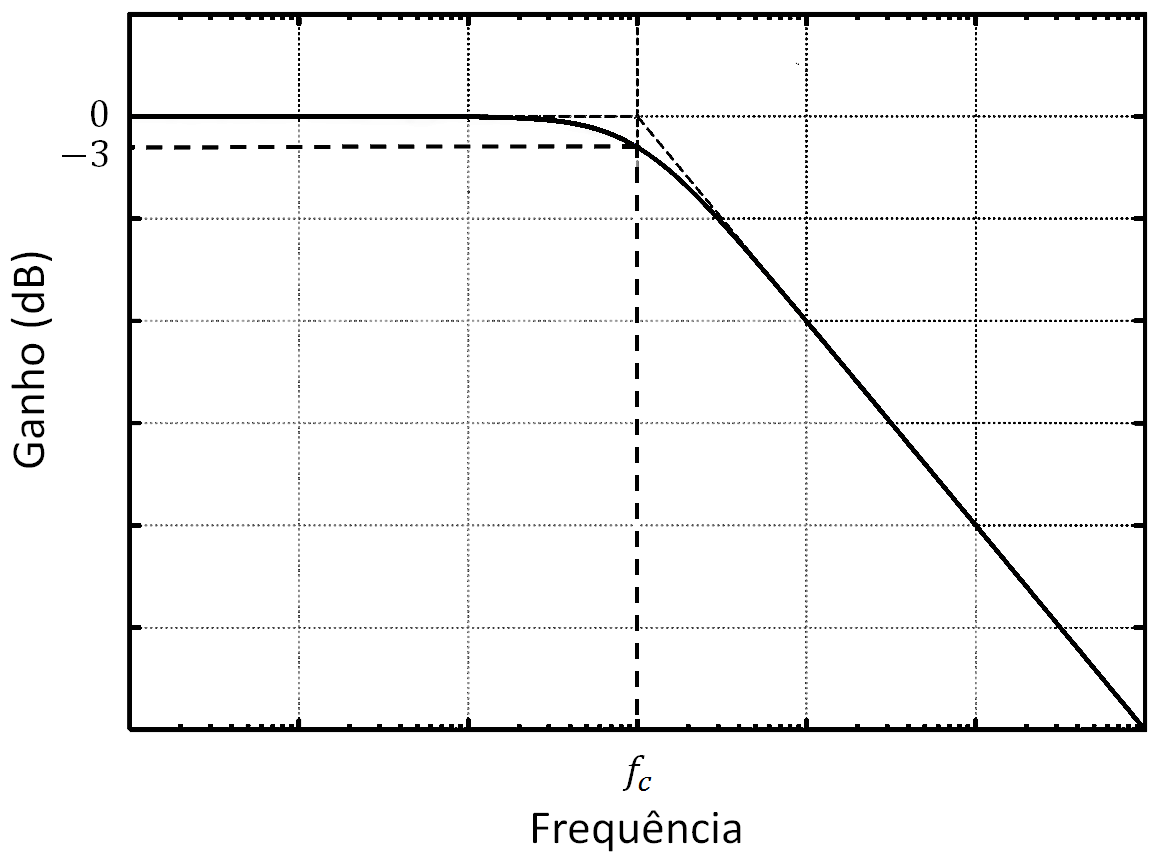
\includegraphics[width=\textwidth]{Cap2/Figuras/LP_filter_BW.png}
			\caption{\centering Resposta em frequência de um filtro passa baixa} 
			\label{fig:LP_filter}
		\end{subfigure}%
		\hfill
		\begin{subfigure}[b]{0.48\textwidth}  
			\centering 
			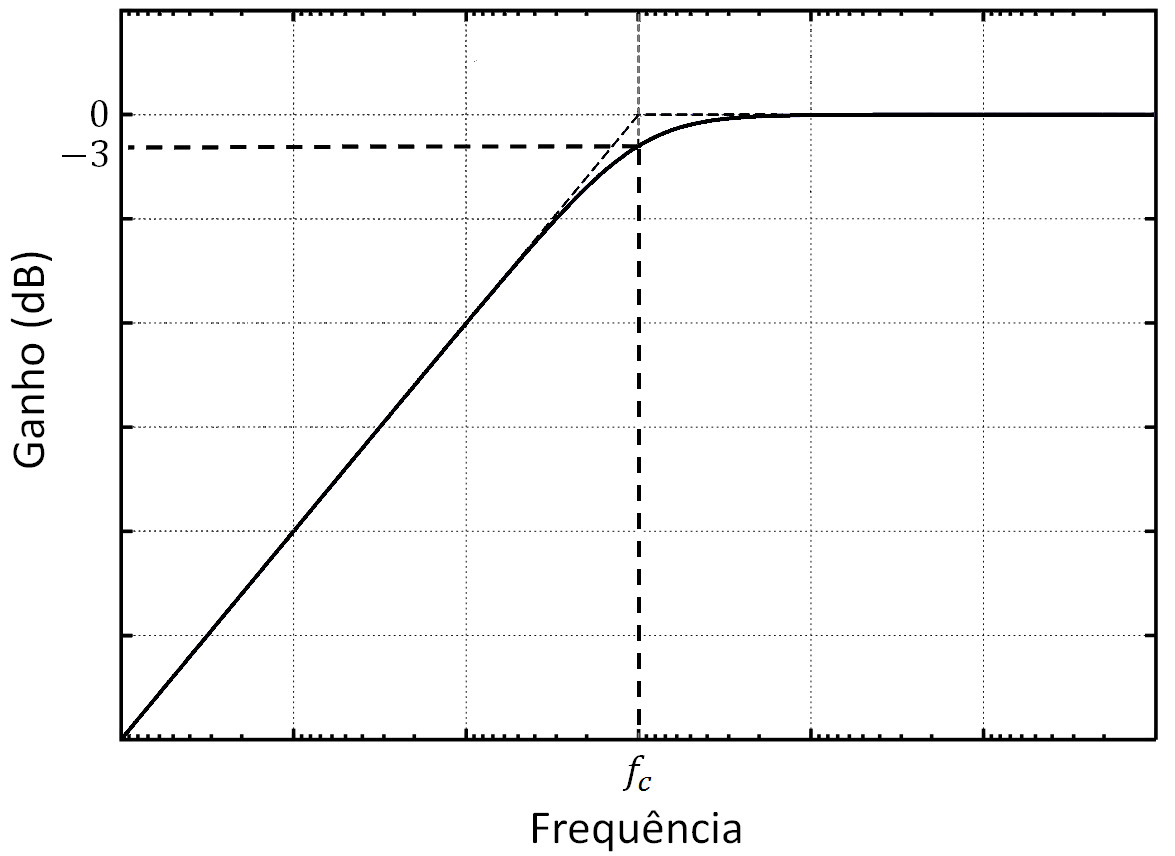
\includegraphics[width=\textwidth]{Cap2/Figuras/HP_filter_BW.png}
			\caption{\centering Resposta em frequência de um filtro passa alta}    
			\label{fig:HP_filter}
		\end{subfigure}%
		\vskip\baselineskip
		\begin{subfigure}[b]{0.48\textwidth}   
			\centering 
			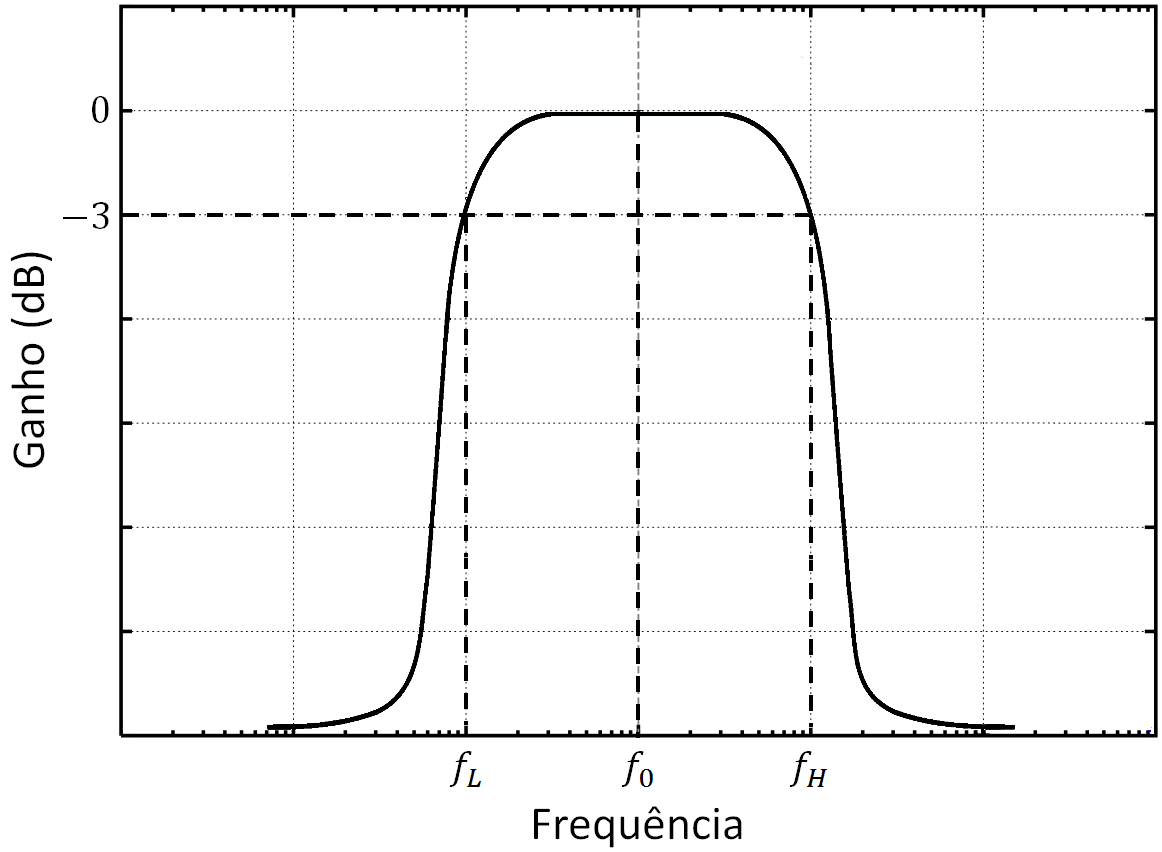
\includegraphics[width=\textwidth]{Cap2/Figuras/BP_filter_BW.png}
			\caption{\centering Resposta em frequência de um filtro passa faixa}   
			\label{fig:BP_filter}
		\end{subfigure}%
		\hfill
		\begin{subfigure}[b]{0.48\textwidth}   
			\centering 
			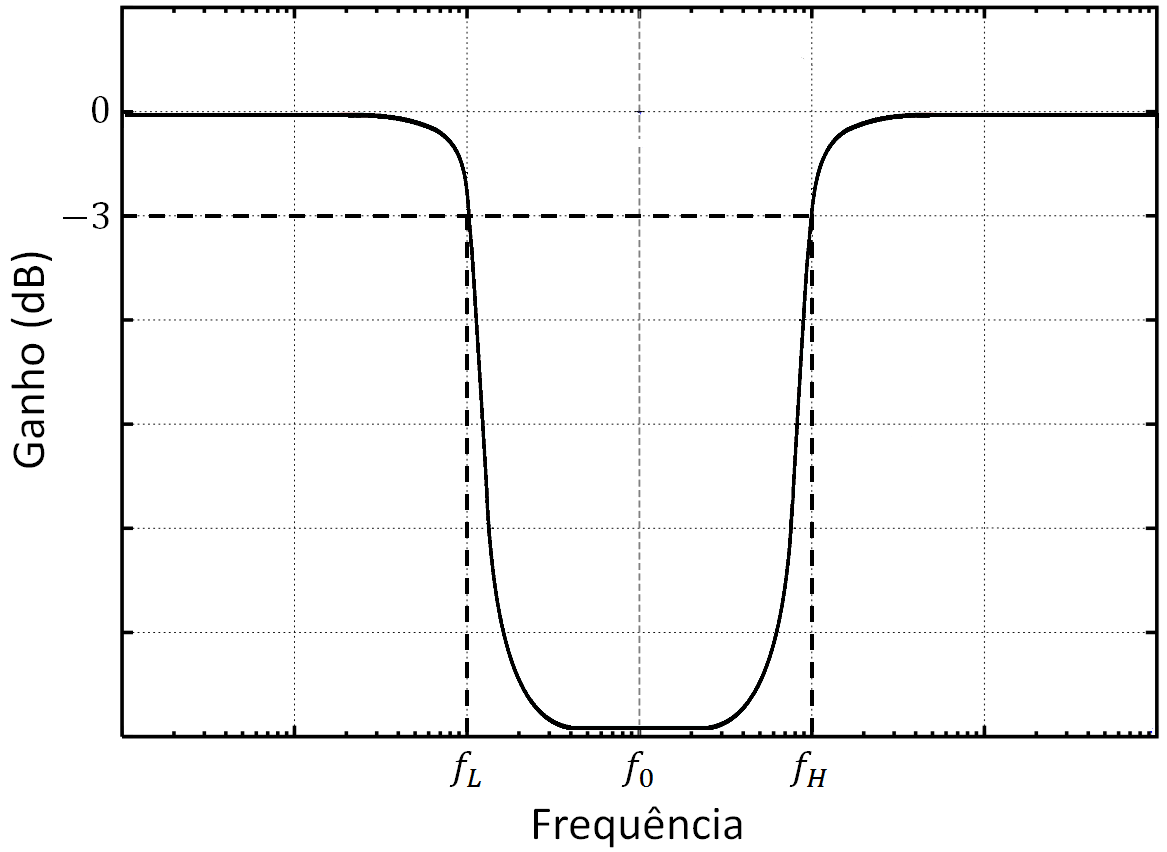
\includegraphics[width=\textwidth]{Cap2/Figuras/RB_filter_BW.png}
			\caption{\centering Resposta em frequência de um filtro rejeita faixa}   
			\label{fig:RB_filter}
		\end{subfigure}%
		\caption{Ganho em função da frequência de filtros passivos típicos} 
		\label{fig:mean and std of nets}
	\end{figure*}
	
\end{enumerate}

Para o problema de atenuar as harmônicas de mais alta frequência que a fundamental, a utilização de filtros passa baixa é mais adequada, pois são os componentes harmônicos que acabam por degradar a qualidade de energia do sistema elétrico.

\subsubsection{Retificadores Multipulso}

Neste tipo de circuito o retificador é concebido utilizando uma filosofia semelhante a um retificador comum com pontes de diodo, porém o arranjo dos semicondutores junto com autotransformadores faz com que a corrente requerida da fonte possua uma forma quase senoidal, tornando o retificador com alto fator de potência. Outra particularidade desse conversor é a ausência de controle externo sobre os semicondutores, sendo que a comutação no retificador ocorre nos diodos e seu funcionamento depende apenas das tensões e correntes aplicadas sob seus terminais.

Os retificadores são comumente encontrados com as topologias dos circuitos partindo de 12 para arranjos de mais pulsos, como 18, 24, 30, ou ainda maiores valores para aumentar a qualidade de energia com relação ao \textit{THD} \cite{Singh2008}. No conceito de operação desse retificador existem autotransformadores na entrada que aplicam tensões e correntes nos terminais dos diodos, onde estes são arranjados de modo que passam a conduzir de forma que a corrente requerida na entrada tenha um formato com baixa incidência de harmônicas de elevada frequência. Ainda, o aumento do número de pulsos do conversor aumenta a qualidade de energia, entretanto eleva a complexidade dos elementos magnéticos do mesmo. Nas figuras \ref{fig:12_pulse} e \ref{fig:18_pulse} são mostrados típicos retificadores de 12 e 18 pulsos, respectivamente, com suas específicas formas de onda. Nessas figuras fica evidente a melhora na forma da corrente senoidal do retificador de 18 pulsos com relação ao de 12 \cite{Singh2008}.

\begin{figure*}[!htbp] %Circuito típico de um retificador de 12 pulsos com sua respectiva corrente de entrada
	\centering
	\begin{subfigure}[b]{0.49\textwidth}
		\centering
		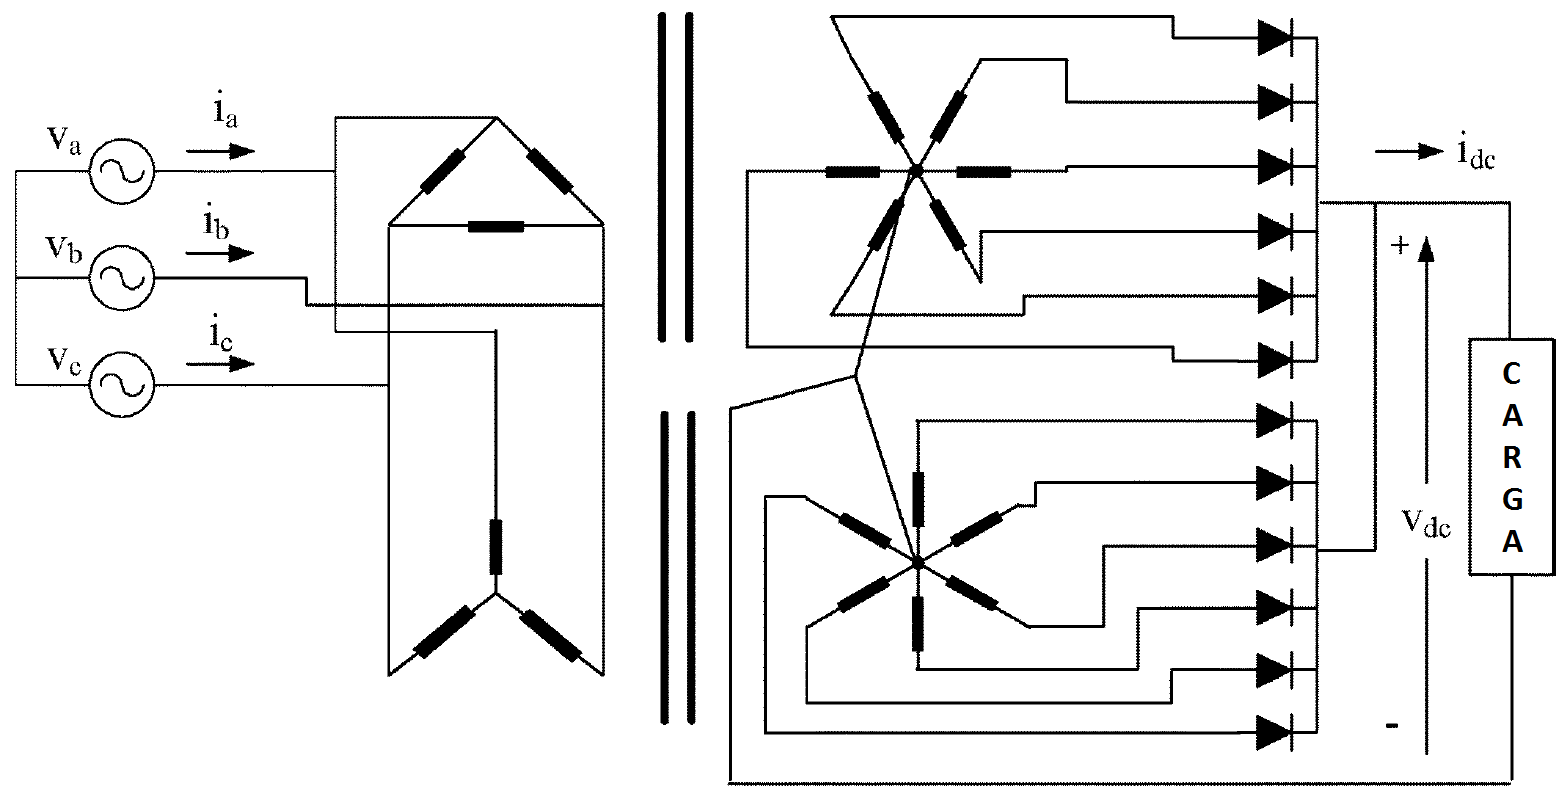
\includegraphics[width=\textwidth]{Cap2/Figuras/12_pulse_rectifier.png}
		\caption{Circuito do retificador de 12 pulsos} 
		\label{fig:12_pulse_rectifier}
	\end{subfigure}%
	\hfill
	\begin{subfigure}[b]{0.49\textwidth}  
		\centering 
		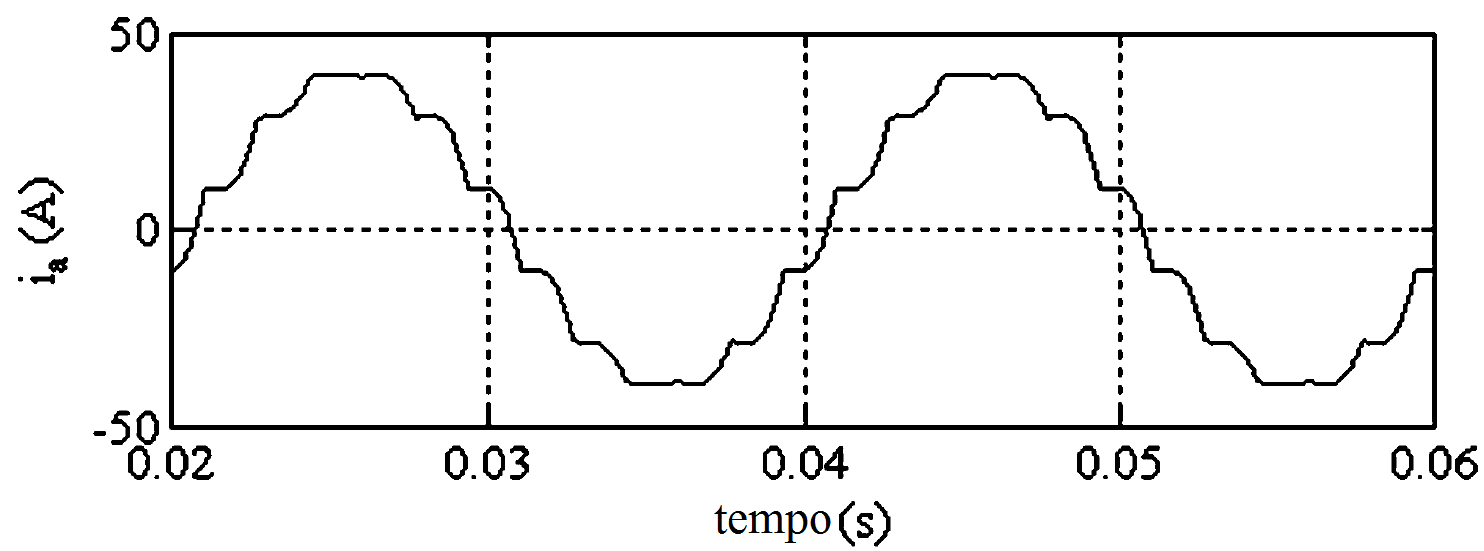
\includegraphics[width=\textwidth]{Cap2/Figuras/12_pulse_wave.png}
		\caption{Forma de onda da corrente de entrada}    
		\label{fig:12_pulse_wave}
	\end{subfigure}%
	\caption{Circuito típico de um retificador de 12 pulsos com sua respectiva corrente de entrada \cite{Singh2008}}
	\label{fig:12_pulse}
\end{figure*}

\begin{figure*}[!htbp] %Circuito típico de um retificador de 18 pulsos com sua respectiva corrente de entrada
	\centering
	\begin{subfigure}[b]{0.49\textwidth}
		\centering
		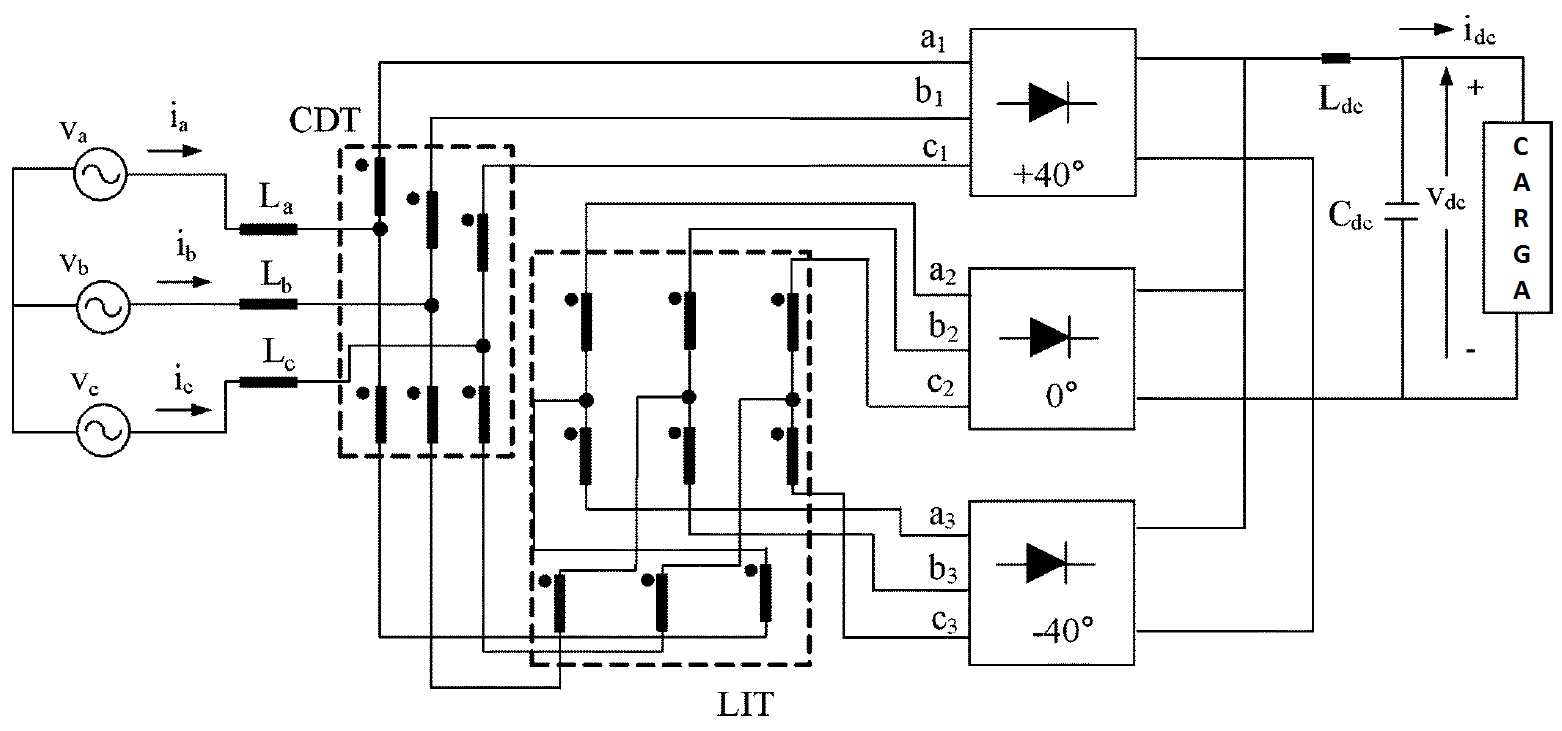
\includegraphics[width=\textwidth]{Cap2/Figuras/18_pulse_rectifier.png}
		\caption{Circuito do retificador de 18 pulsos} 
		\label{fig:18_pulse_rectifier}
	\end{subfigure}%
	\hfill
	\begin{subfigure}[b]{0.49\textwidth}  
		\centering 
		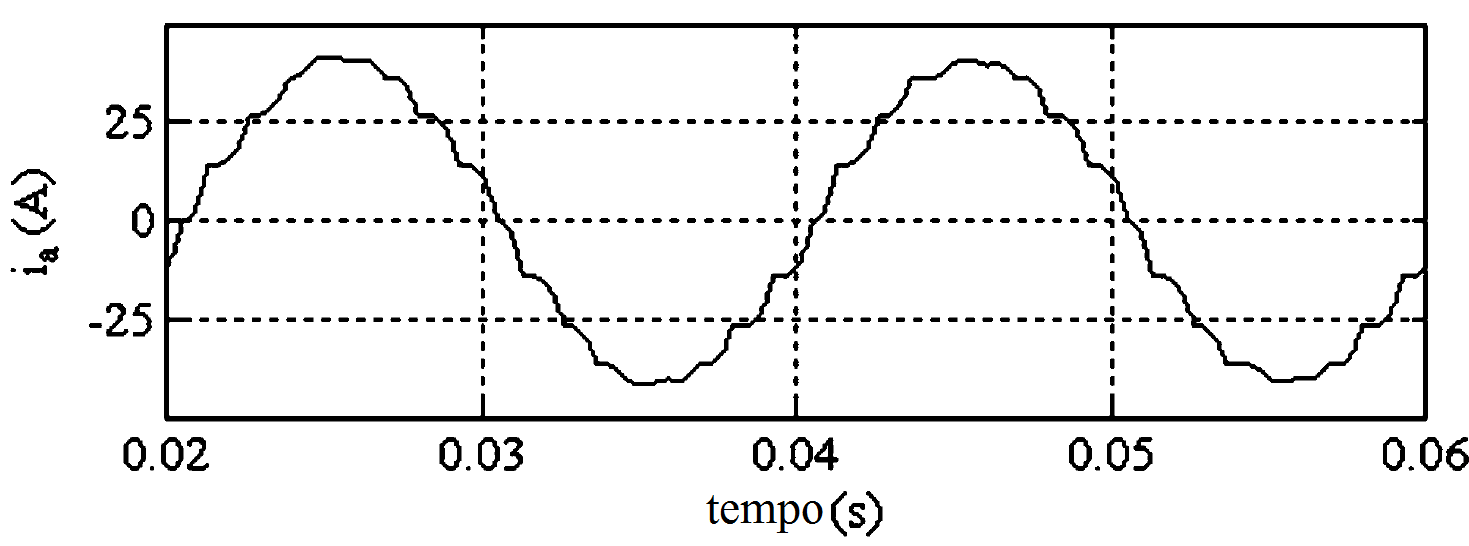
\includegraphics[width=\textwidth]{Cap2/Figuras/18_pulse_wave.png}
		\caption{Forma de onda da corrente de entrada}    
		\label{fig:18_pulse_wave}
	\end{subfigure}%
	\caption{Circuito típico de um retificador de 18 pulsos com sua respectiva corrente de entrada \cite{Singh2008}}
	\label{fig:18_pulse}
\end{figure*}

Cabe lembrar que a utilização de retificadores multipulso é realizável tanto em redes de 60 Hz quanto em sistemas de elevada frequência, como 400-800 Hz \cite{Gong2003,Lobo2005}. Isto faz-se necessário para atender o mercado aeronáutico que possui o sistema elétrico operando em 400 Hz, ou ainda, até 800 Hz para geração em frequência variável.

\subsection{Sistemas Ativos}

Em sistemas ativos a retificação é feita com a utilização de conversores operados com a implementação de chaves estáticas com comutação controlada, cujo objetivo é diversificar as topologias e, dentro de certas faixas de operação, reduzir as perdas por condução quando comparados com circuitos comutados por diodos. Com isso, a flexibilidade de projeto é aumentada de modo que há uma maior diversificação de tipos de retificadores disponíveis. Além do mais, com o comando na comutação é possível haver uma melhor regulação da tensão na saída do sistema e, utilizando certas topologias, um controle de corrente de entrada de modo a proporcionar um fator de potência em acordo com os requisitos de qualidade de energia do sistema. Dois dos principais tipos de sistemas ativos implementados para mitigar as harmônicas da rede são os conversores de alto fator de potência e os filtros ativos.

\subsubsection{Conversores com Correção de Fator de Potência}

A topologia de um conversor regulado com correção de fator de potência está inserida em retificadores com condicionamento de dois estágios. A operação desses retificadores tem em seu primeiro estágio a conversão AC-DC da tensão, seguido de um segundo estágio com a regulação dos níveis DC para valores bem definidos de tensão \cite{Kolar2011}. A figura \ref{fig:rectifier_sch} mostra o esquema de um conversor de dois estágios. Usualmente o primeiro estágio é concebido pelo arranjo de uma ponte retificadora à diodo, como mostra a figura \ref{fig:3ph_rectifier}. Esse tipo de retificador, por sua simplicidade, possui um baixo fator de potência com alta distorção de corrente na linha de entrada. Para contornar este problema, conversores AC-DC com correção de fator de potência são empregados no primeiro estágio de condicionamento, tendo o controle de distorção harmônica com a inserção de semicondutores com comutação controlada. O controle de fator de potência dá-se com a operação de comando dos comutadores de forma que a corrente de entrada do conversor rastreie a forma de onda da tensão da rede, proporcionando um alto FP. \cite{Kolar2011,Barbosa2002}.

\begin{figure}[!htbp] % Conversores AC-DC de dois estágios
	\centering
	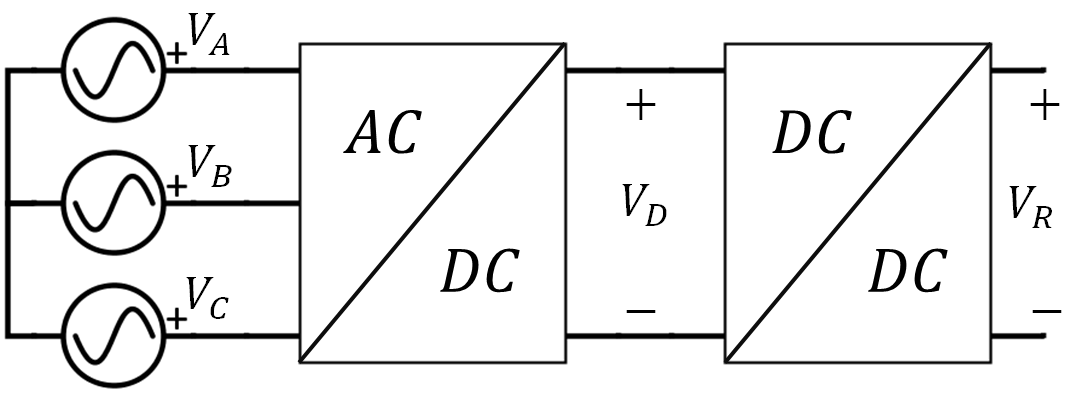
\includegraphics[width=0.4\textwidth]{Cap2/Figuras/rectifier_sch.png}
	\caption{Conversores AC-DC de dois estágios}
	\label{fig:rectifier_sch}
\end{figure}

\begin{figure}[!htbp] % Retificador trifásico com ponte de diodos
	\centering
	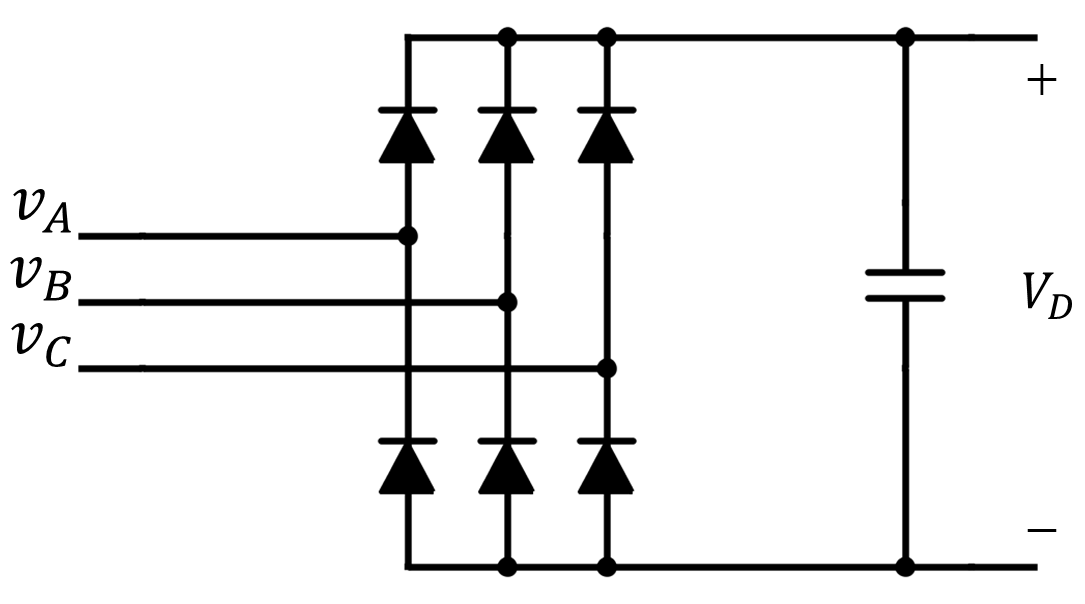
\includegraphics[width=0.45\textwidth]{Cap2/Figuras/3ph_rectifier.png}
	\caption{Retificador trifásico com ponte de diodos}
	\label{fig:3ph_rectifier}
\end{figure}

Encontram-se inúmeras topologias de conversores com correção de fator de potência na literatura. O mais utilizado é o conversor com correção de fator de potência, ou \textit{Power Factor Correction} (PFC) do tipo \textit{boost}. Esse conversor é concebido pela ponte de diodos arranjados juntamente com chaves controladamente comutadas. Ainda, pela flexibilidade de possíveis arranjos dos semicondutores sob a ponte de diodos e pelas linhas de entrada e saída de energia, uma gama imensa de conversores do tipo \textit{PFC boost} pode ser concebido. Para elucidar o funcionamento deste tipo de conversor será estudado o circuito Prasad-Ziogas (figura \ref{fig:PFC_converter}), cuja topologia é simples e apresenta uma única chave controlada. Também para facilitar o entendimento, será explicado a operação em modo de condução descontínua. O princípio de funcionamento é dado pelo controle da chave $S_1$ que, quando em estado de condução, aplica a tensão da fonte sobre os indutores de entrada $L_i,\;i=1,2,3$. Isso faz com que as correntes nos indutores cresçam de forma proporcional a tensão aplicada em seus terminais pela fonte de entrada. Quando o a chave $S_1$ para de conduzir, as correntes dos indutores são levadas à zero. Por ter a frequência de comutação muito maior que a frequência da rede, tem-se que a corrente de entrada apresenta uma forma modulada em alta frequência e facilmente filtrada com filtros passa-baixo \cite{Nairus1996, Takeuchi2008}. Com isso é possível que a corrente apresente formato senoidal e em fase com a tensão. Na prática o funcionamento desse conversor apresenta certa distorção harmônica e não suporta alta capacidade de potência, de modo que outras topologias hibridas com circuitos \textit{PFC boost} e \textit{PFC buck} sejam utilizadas, ou ainda, pelo controle individual do fator de potência de cada fase para aumentar a capacidade de condicionamento de energia e tornar o FP próximo da unidade \cite{Kolar2011}.

\begin{figure}[!htbp] %Conversor com correção de fator de potência do tipo Prasad-Ziogas \cite{Takeuchi2008}
	\centering
	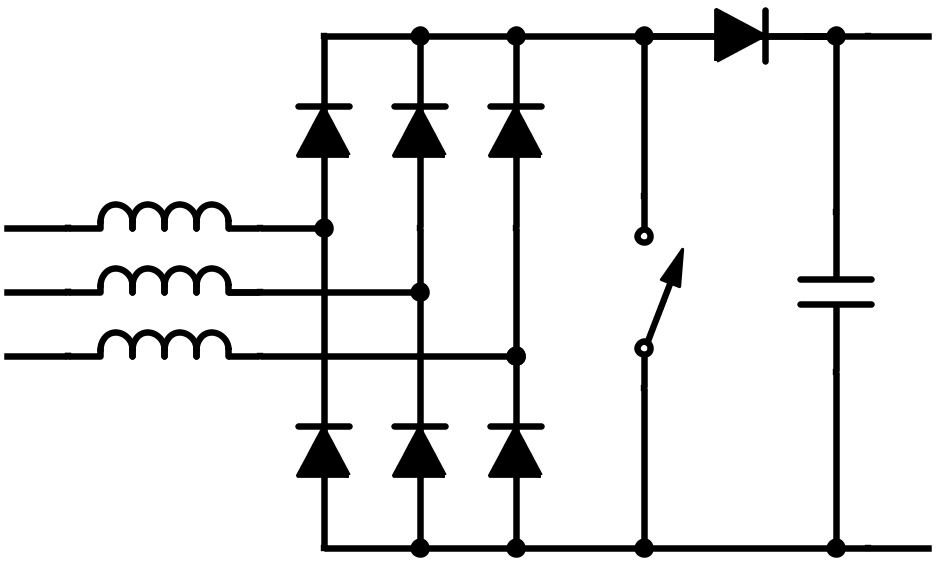
\includegraphics[width=0.45\textwidth]{Cap2/Figuras/PFC_converter.png}
	\caption{Conversor com correção de fator de potência do tipo Prasad-Ziogas \cite{Takeuchi2008}}
	\label{fig:PFC_converter}
\end{figure}

%\begin{figure*}[!htbp] 
%	\centering
%	\begin{subfigure}[b]{0.45\textwidth}
%		\centering
%		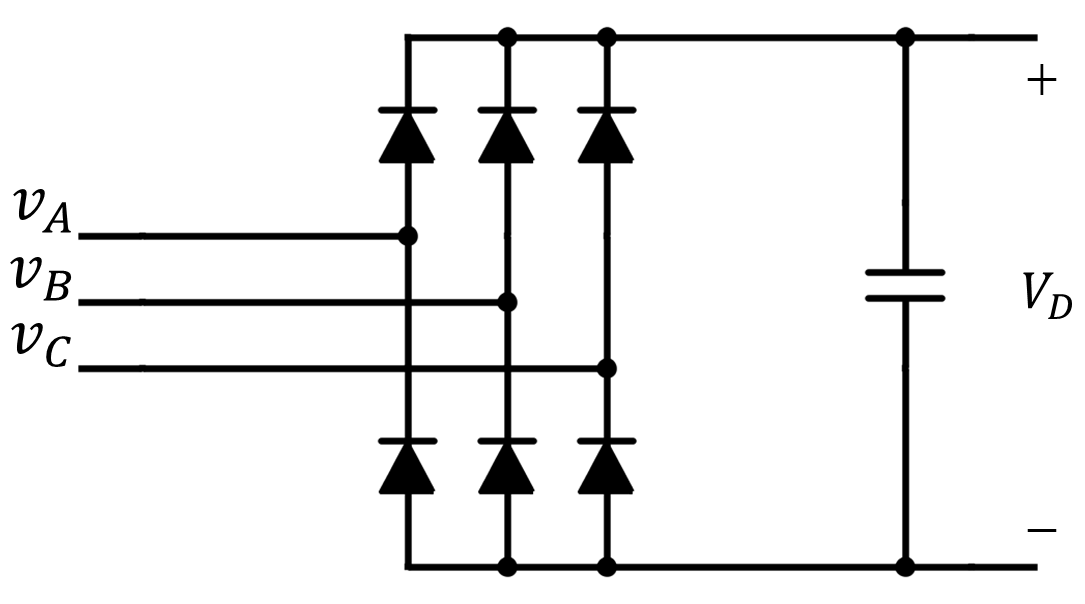
\includegraphics[width=\textwidth]{Cap2/Figuras/3ph_rectifier.png}
%		\caption{Retificador trifásico com ponte de diodos} 
%		\label{fig:3ph_rectifier}
%	\end{subfigure}%
%	\hspace{0.45cm}
%	\begin{subfigure}[b]{0.45\textwidth}  
%		\centering 
%		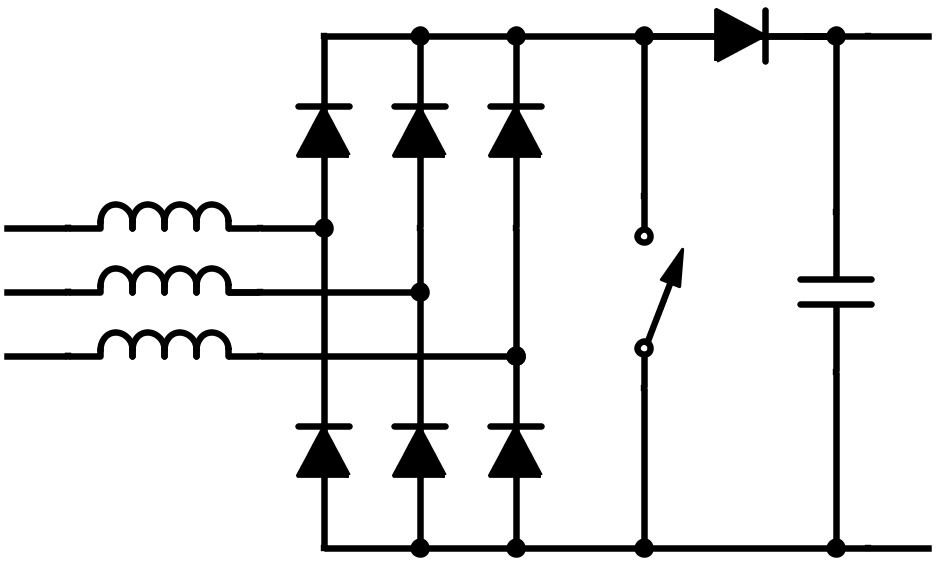
\includegraphics[width=\textwidth]{Cap2/Figuras/PFC_converter.png}
%		\caption{Conversor com correção de fator de potência do tipo Prasad-Ziogas \cite{Takeuchi2008}}    
%		\label{fig:PFC_converter}
%	\end{subfigure}%
%	\caption{}
%	\label{fig:rectifiers}
%\end{figure*}

Como resultado da operação do conversor Prasad-Ziogas, as formas de onda nos indutores de entrada são tidos como mostrado na figura \ref{fig:PFC_waveforms}. Como mencionado, a forma de onda apresenta modulação em amplitude (figura \ref{fig:PFC_unfilt}), assim o espectro de frequência da corrente de entrada apresenta um pico de alto valor na fundamental juntamente com harmônicas nas altas frequências. Como consequência, é possível implementar filtros passa-baixo com a alta frequência de corte nas linhas da rede, de modo que as harmônicas sejam atenuadas, sobrando apenas a componente fundamental. A corrente de linha resultante após a filtragem é mostrado na figura \ref{fig:PFC_filt}.

\begin{figure*}[!htbp] % Corrente de entrada para o caso sem e com filtro na linha
	\centering
	\begin{subfigure}[b]{0.499\textwidth}
	\centering
	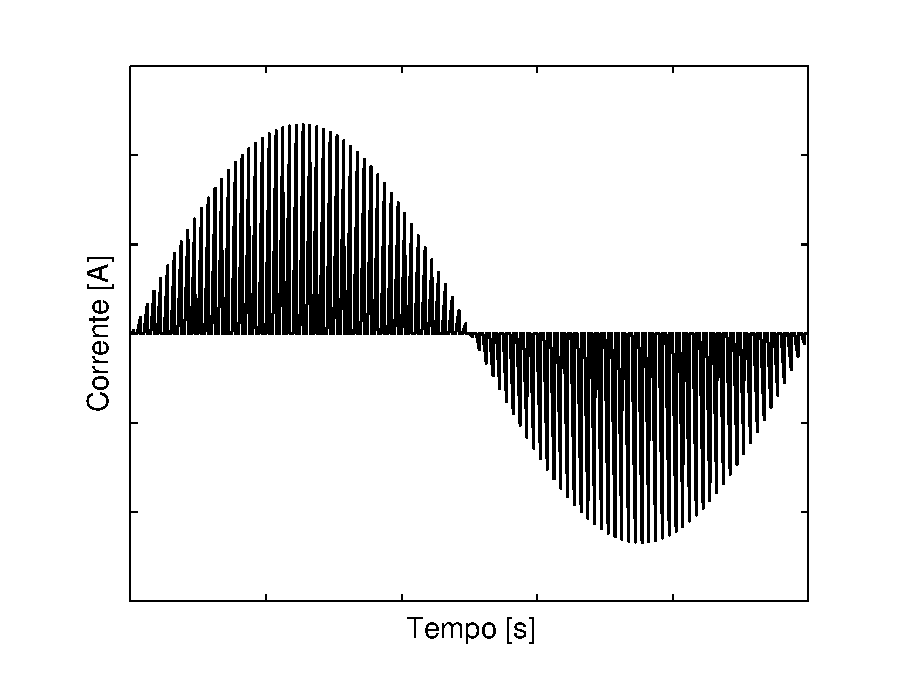
\includegraphics[width=\textwidth]{Cap2/Figuras/PFC_unfilt.eps}
	\caption{Corrente dos indutores de entrada sem filtragem}
	\label{fig:PFC_unfilt}
	\end{subfigure}%
	\hfill
	\begin{subfigure}[b]{0.499\textwidth}  
		\centering 
		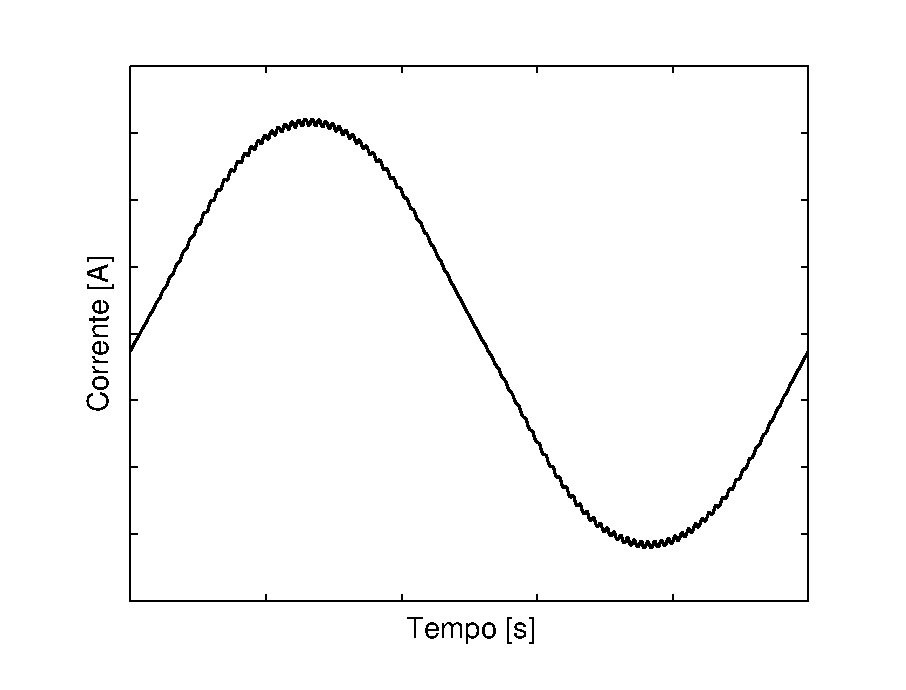
\includegraphics[width=\textwidth]{Cap2/Figuras/PFC_filt}
		\caption{Corrente dos indutores de entrada  com filtragem de 2º ordem}    
		\label{fig:PFC_filt}
	\end{subfigure}%
	\caption{Corrente de entrada para o caso sem e com filtro na linha}
	\label{fig:PFC_waveforms}
\end{figure*}
\todo{Arrumar espessura da linha da figura (a)}
\subsubsection{Filtros Ativos}

Filtros ativos podem ser classificados em dois tipos: os baseados em amplificadores operacionais e os baseados em conversores CC-CA. O princípio de funcionamento do primeiro tipo de filtro é igual em sistema passivo, onde a operação é dada pela atenuação de determinadas componentes de frequência da rede. A diferença desse tipo de filtros ativos com os passivos é que no primeiro há a presença de amplificadores operacionais, a qual necessitam de fontes externas para funcionar adequadamente. Esse tipo de filtragem é muito utilizado em sinais de baixa potência, sendo que para o escopo desse trabalho torna-se inviável dado o tipo de potência do sistema elétrico de aeronaves. 

A filtragem baseada em conversores CC-AC tem por princípio a utilização de inversores controlados, visto que este tipo de conversor pode, teoricamente, recriar formas de tensão e corrente de qualquer configuração dada à uma referência definida\cite{Pomilio2009}. O princípio dos filtros ativos é promover a qualidade de energia pela compensação das componentes harmônicas presentes nos sistemas quando há a conexão de cargas não lineares. Ainda, pode-se corrigir o fator de potência de deslocamento com a filtragem ativa. Os filtros ativos baseados em conversores CC-CA possuem topologias de tal forma à compensar a não linearidade da corrente da carga ou a distorção na forma de tensão do barramento com a utilização de filtros \textit{shunt} ou filtros série, respectivamente. O funcionamento do primeiro tipo de filtro é dado pela injeção de corrente na rede que, somado com a requerida pela carga, faz com que a corrente no barramento do gerador tenha forma de onda senoidal e em fase com a tensão. A consequência do uso desse filtro reflete tanto no fator de potência como também na distorção harmônica na forma de onda de tensão no barramento de geração \cite{Afonso2013}, visto que não haverá quedas de tensão de forma distorcidas nas reatâncias dos geradores e linhas de transmissão. Um exemplo de funcionamento de uma filtro \textit{shunt} pode ser visto na figura \ref{fig:shunt}, onde é mostrado as formas de onda de corrente na carga e no filtro que, quando somadas, tem como produto a forma sinusoidal de corrente nas linhas de transmissão. Já o filtro série tem como objetivo a correção da distorção da tensão aplicada à carga com a inserção de fontes controlada de tensão na linha de alimentação. A compensação dá-se pela adição de componentes defasadas em 180° às harmônicas geradas pela distorção de corrente sobre as reatâncias das linhas. Para esse último filtro a forma de onda da corrente não é compensada, de modo que o fator de potência não é igual a unidade. Assim, tem-se que o filtro série é indicado apenas para assegurar a forma de onda senoidal de tensão no lado de alimentação da carga \cite{Afonso2013}. A figura \ref{fig:serie} mostra um filtro ativo série em um sistema. Nota-se que a tensão pelo lado do barramento de geração e distribuição é distorcida, porém com a adição das tensões $V_{Ac}$, $V_{Bc}$ e $V_{Cc}$ em suas respectivas linhas, as tensões na entrada da carga apresentam uma forma de onda senoidal pura. A utilização desse tipo de filtro é apenas indicada quando deseja-se preservar a integridade da qualidade de energia pelo lado da carga, visto que a carga ainda apresenta injeção corrente distorcida no sistema de modo a contribuir com a má qualidade de energia da rede.

\begin{figure}[!htbp]
	\centering
	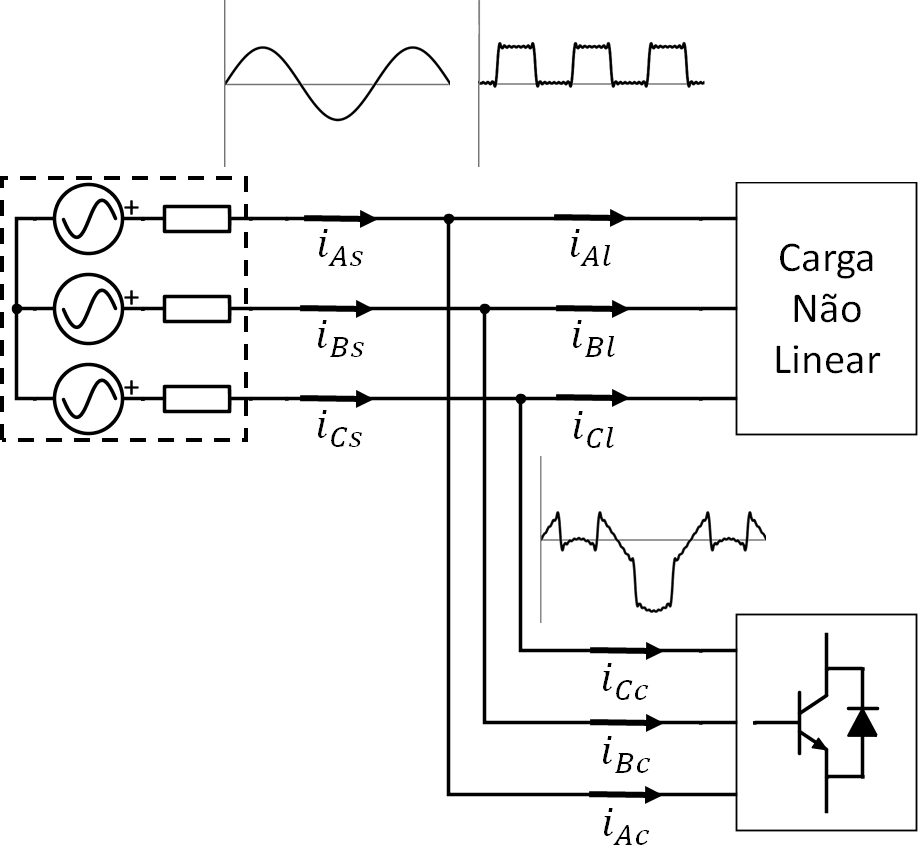
\includegraphics[width=0.5\textwidth]{Cap2/Figuras/shunt.png}
	\caption{Filtro ativo do tipo \textit{shunt}}
	\label{fig:shunt}
\end{figure}

\begin{figure}[!htbp] %width = width_shunt*1.1335
	\centering
	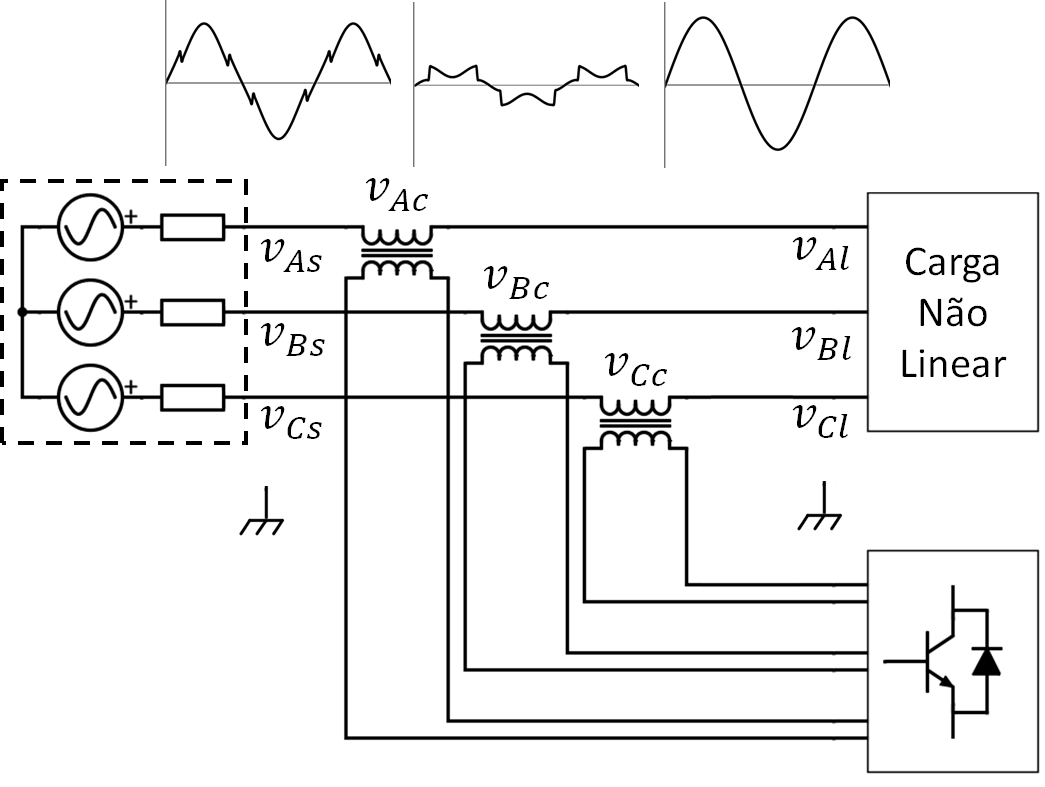
\includegraphics[width=0.567\textwidth]{Cap2/Figuras/serie.png}
	\caption{Filtro ativo do tipo série}
	\label{fig:serie}
\end{figure}

Em um sistema elétrico genérico com a presença de cargas lineares e/ou não pode-se garantir a qualidade de energia de todo o sistema com a correção da forma de onda da corrente de todos os pontos de entrada de carga. Caso o sistema não possua essa característica para correção da qualidade de energia, mas seja desejado que uma nova carga não interfira no sistema e, além disso tenha uma forma de onda de tensão pura em seus terminais, pode-se utilizar a topologia híbrida, onde há a presença tanto do filtro \textit{shunt} quanto série num mesmo ponto de alimentação. Com isso, tem-se que possíveis distorções da tensão são corrigidas pelo filtro série, e ainda, garante-se que a corrente dessa carga não interfira no resto do sistema com relação a baixa qualidade de energia.

\section{Vantagens e Desvantagens dos Sistemas de }\todo{Melhorar o título visto que alguns métodos não atenuam e sim já implementam a solução com alto fator de potência}

\begin{figure}[!htbp]
	\centering
	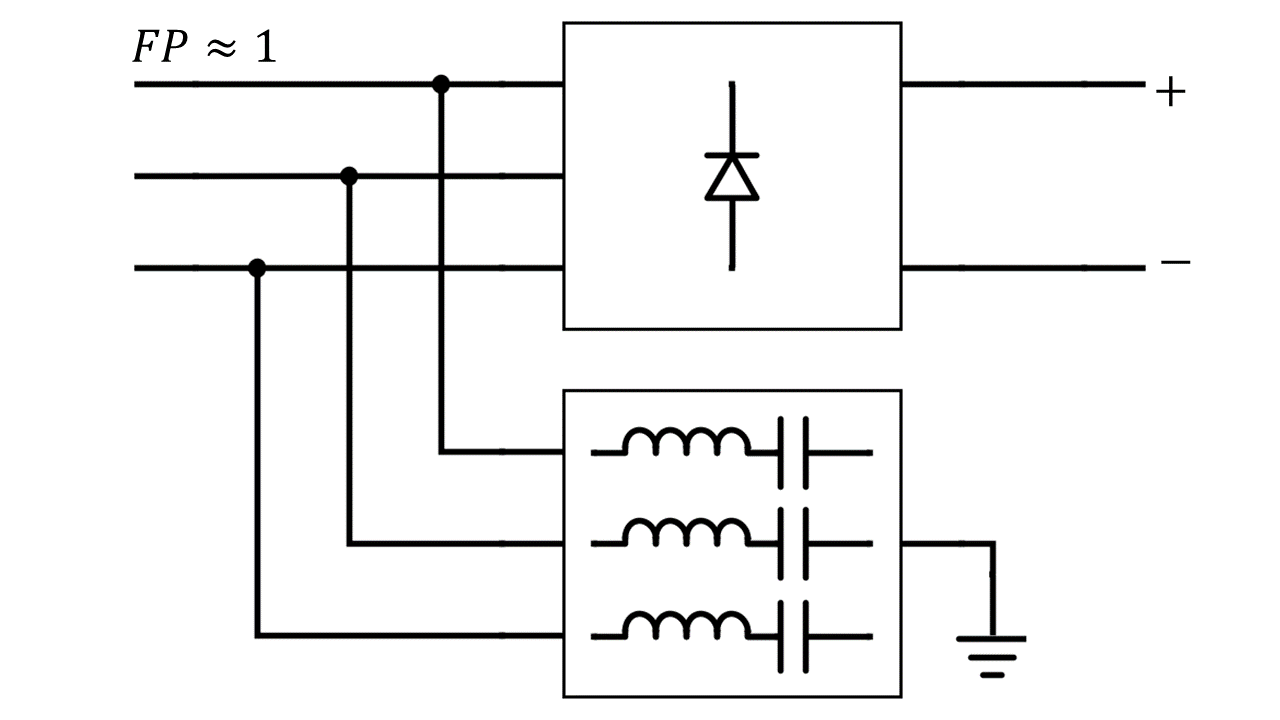
\includegraphics[width=0.55\textwidth]{Cap2/Figuras/sch_filtro_passivo.png}
	\caption{Filtro Passivo}
	\label{fig:sch_filtro_passivo}
\end{figure}

\begin{figure}[!htbp]
	\centering
	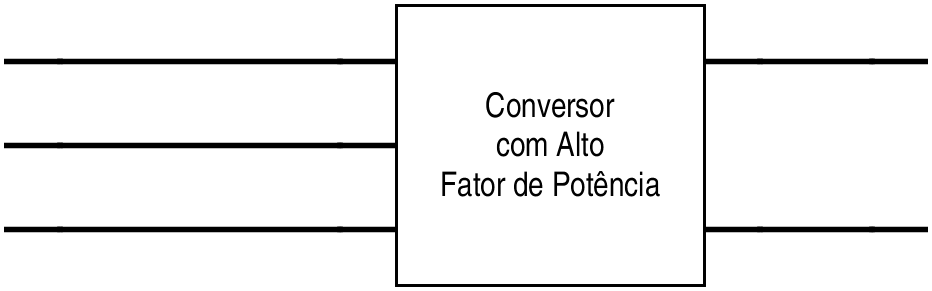
\includegraphics[width=0.55\textwidth]{Cap2/Figuras/sch_PFC.png}
	\caption{Conversor PFC}
	\label{fig:sch_PFC}
\end{figure}

\begin{figure}[!htbp]
	\centering
	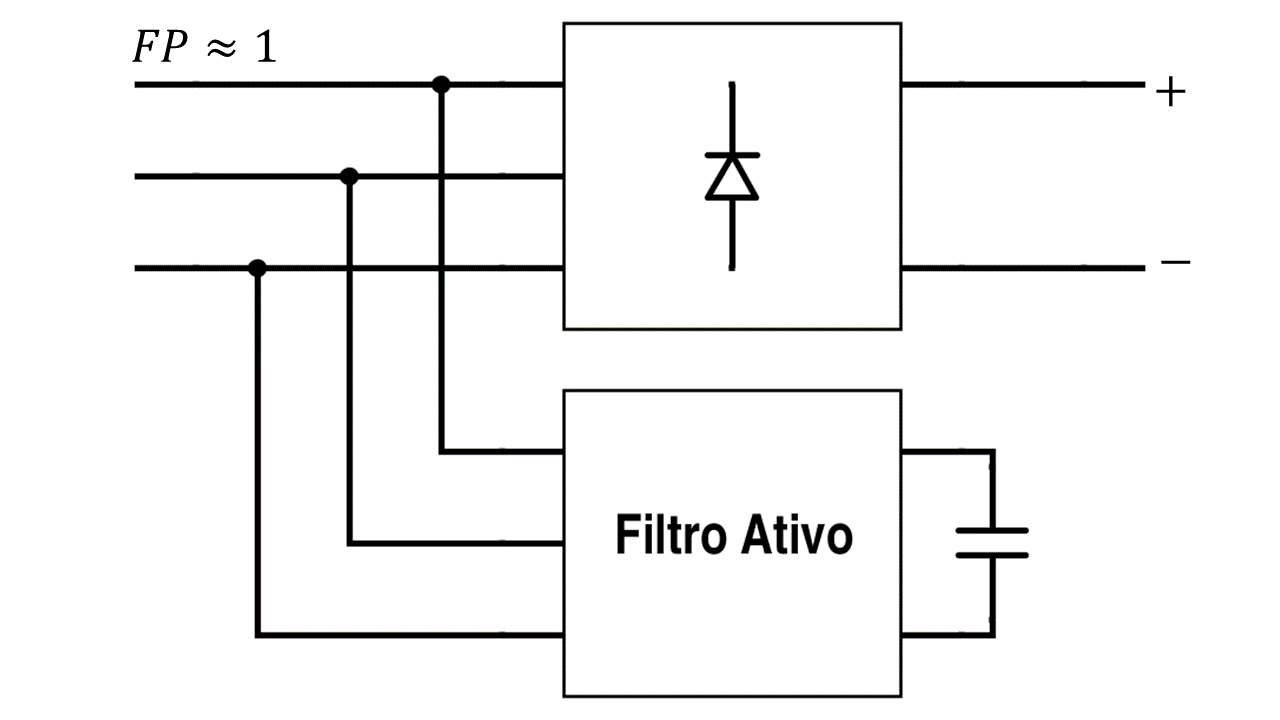
\includegraphics[width=0.55\textwidth]{Cap2/Figuras/sch_filtro_ativo.png}
	\caption{Filtro Ativo}
	\label{fig:sch_filtro_ativo}
\end{figure}




